\section{Constructing a Benchmark Dataset}
In this section, we provide a detailed explanation of our task, which involves assessing whether a given user's query is answerable in RaCG (\textsection 2.1). We also describe how we constructed the benchmark dataset, RaCGEval, to evaluate the performance of models in solving this task (\textsection 2.2, \textsection 2.3, and \textsection 2.4), and discuss the reliability of this dataset (\textsection 2.4).

\begin{figure*}[t!]
    \centering
    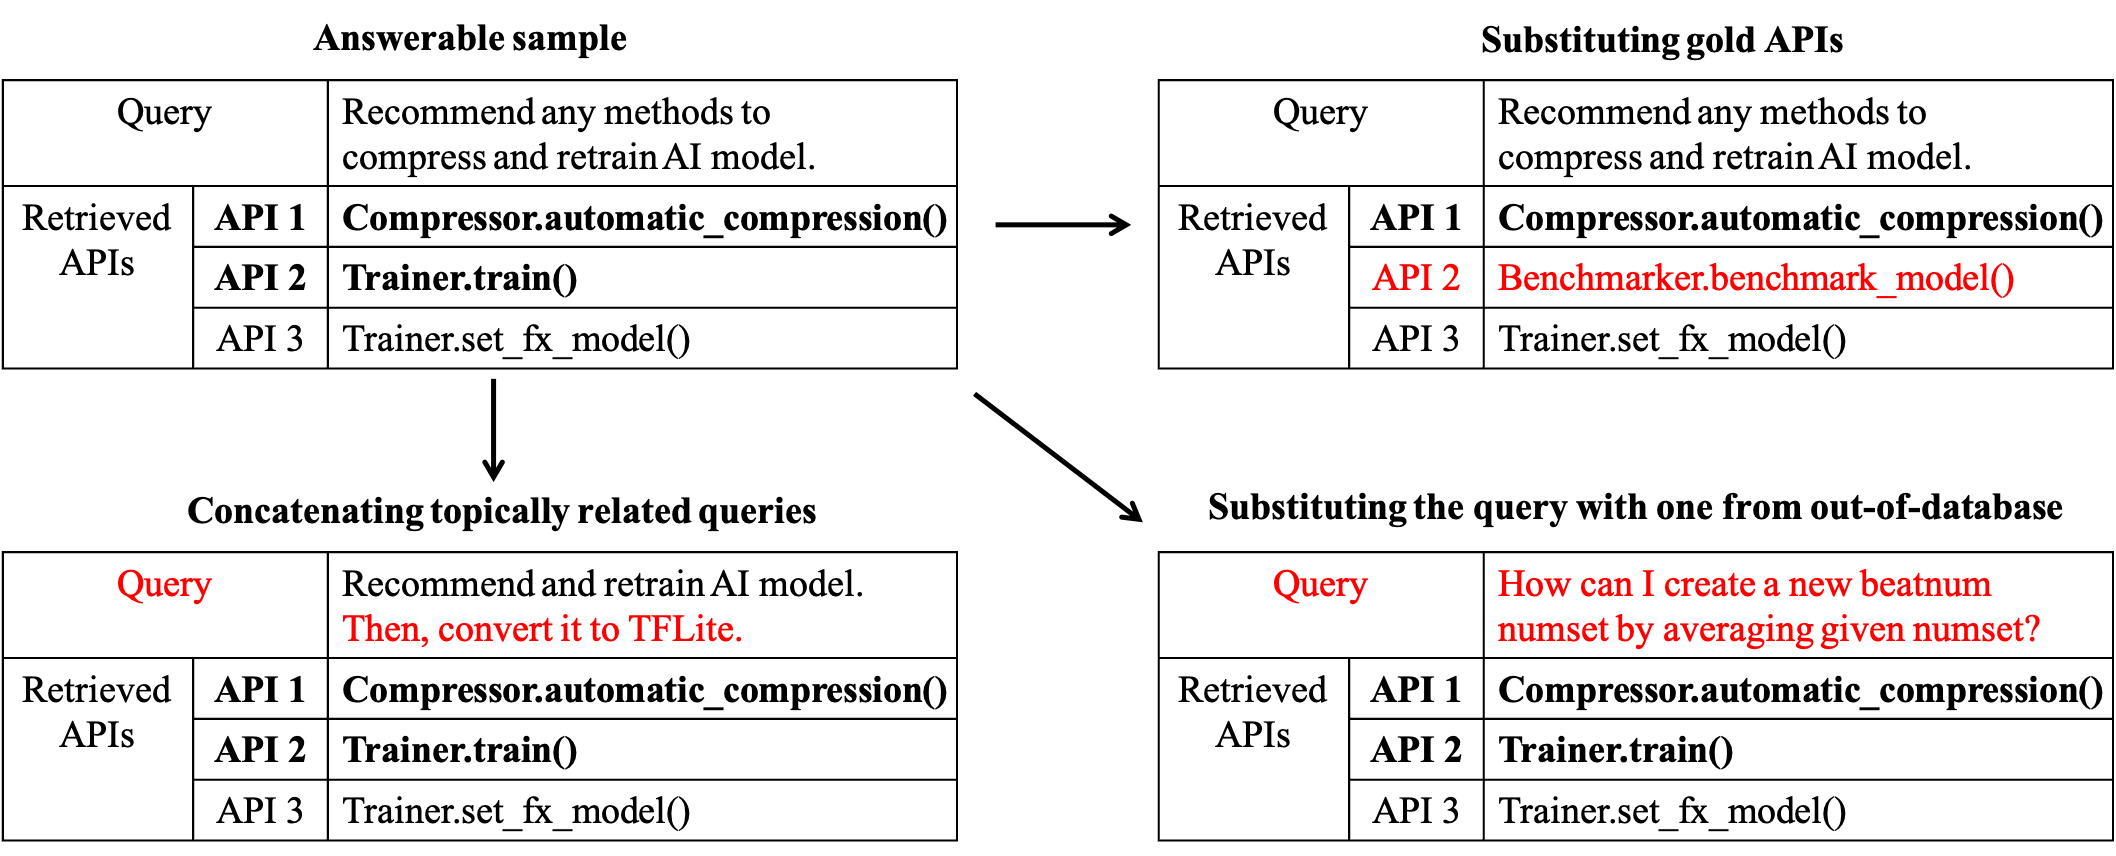
\includegraphics[width=1.0\linewidth]{figures/fig_3.png}
    \caption{Examples of NegGen method to build unanswerable/partially answerable samples. The API highlighted in bold is the gold API for the given query in the answerable set.}
    \label{fig:3}
\end{figure*}



\subsection{Task description}
\label{sec:2_1}
Assessing the answerability of users' queries in the RaCG involves determining whether correct codes can be derived solely from the information provided in the input prompts. As depicted in Figure~\ref{fig:2}, each input prompt is created by combining a user's query with relevant APIs extracted from the target API documentation associated with that query. Each query typically consists of a single request, but it can sometimes contain multiple requests that share similar topics. Accordingly, if all requests can be answered through the extracted API descriptions, the query can be considered \textbf{answerable}. If only some requests can be resolved, it can be deemed \textbf{partially answerable}. If none of the requests can be resolved, it can be regarded as \textbf{unanswerable}. In conclusion, our task can be viewed as a three-way classification problem that takes an input prompt (i.e., instruction for answerability assessment with pairs of a user query and API descriptions) as input.

\subsection{API documentation}
\label{sec:2_2}
In our task, the language model must be able to determine whether an answer can be provided based solely on the information in the given input prompt. Therefore, to ensure a fair assessment that excludes prior knowledge of each LLM, the benchmark dataset includes APIs that most language models are unlikely to have encountered during training. Therefore, we use the following datasets that contain private or modified API information:

\begin{itemize}
  \item NetsPressoEval~\cite{netspresso2024}: The API documentation of NetsPresso, a deep learning model optimization platform, includes functions for compressing deep learning models or compiling them for specific hardware
  \item TorchDataEval~\cite{zan-etal-2022-language}: A collection of API descriptions for TorchData, which is a beta library for a modular data loading framework and efficient data pipelines
  \item BeatNumEval~\cite{zan-etal-2022-language}: The API documentation for Python NumPy, with its keywords and structure rephrased
  \item MonkeyEval~\cite{zan-etal-2022-language}: The API documentation for Python Pandas, with its keywords and structure rephrased
\end{itemize}
The other three datasets, excluding NetsPressoEval, are datasets studied in previous research~\cite{zan-etal-2022-language, zan2023privatelibrary}. Each sample in these datasets consists of a user's query and the retrieved APIs with a description. We manually add gold APIs, which can address user queries, if not presented in retrieved APIs. Each sample can be viewed as an answerable input prompt. Unlike the other datasets, NetsPressoEval is a newly created dataset for this study, and the answerable input prompts were generated by consulting those who develop the APIs. An example of the dataset for NetsPressoEval can be found in Table~\ref{tab:3} in Appendix~\ref{appendix:a}. 

\subsection{Generating partially answerable and unanswerable samples}
\label{sec:2_3}

So far, we have only been able to obtain answerable samples. Here, we propose a method to generate partially answerable and unanswerable samples using the answerable samples.

Currently, each answerable sample consists of a query ($q^*$)
and retrieved APIs ($\hat{R}=\{\hat{r}_1,\hat{r}_2,...\}$). The retrieved APIs also include gold APIs ($R^*=\{r_1^*, r_2^*, ...\}$). In this study, all samples are limited to having three retrieved APIs for a single query. This is to account for the input length limitations of many language models (i.e., 8192 tokens for llama-3-7B) and prompt length increases with the number of APIs included. The APIs associated with each query are determined based on their similarity scores to the query, in descending order. We denote the final selected APIs as $R=\{r_1, r_2, r_3\}$. We generated partially answerable and unanswerable samples using the following methods:
\begin{itemize}
  \item Substituting the gold APIs: To generate partially answerable and unanswerable samples, we substitute $r_i^* \in R^*$ with $\hat{r_j}$ such that $S(q^*, \hat{r_j})\geq\tau_{r}$, $\hat{r_j} \notin R^*$ and $\hat{r_j} \notin R$. $S( , )$ is the similarity score between two descriptions, which is measured in our study using the encoder of CodeT5+~\cite{wang-etal-2023-codet5}. $\tau_{r}$ and $\tau_{i}$ are the relevant and irrelevant thresholds. In this study, we use $\tau_{r}=0.8$, and $\tau_{i}=0.1$. In other words, it involves replacing the gold APIs with APIs that are semantically similar to the query but do not assist in generating the code corresponding to that query. If all gold APIs are replaced, the sample becomes an unanswerable sample. However, if only some are replaced, it becomes a partially answerable sample because certain request requirements in the query cannot be fulfilled.
  \item Concatenating topically related queries: To obtain partially answerable samples, we concatenate $q^*$ with $q$ such that $S(q,q^*)\geq\tau_{r}$ and $S(q,r^*)<\tau_{i}$. Here, $q$ refers to one of the queries included in the dataset related to the same API documentation. The newly added queries are unrelated to the gold APIs and therefore cannot be resolved. As a result, these samples become partially unanswerable samples.   
  \item Substituting the query with one from out-of-database: To generate unanswerable samples, we substitute $q^*$ with $q$ such that $S(q,r^*) < \tau_{i}$. The $q$ comes from other datasets.
\end{itemize}
Our methods are well illustrated in Figure~\ref{fig:3}. 

\subsection{Annotation}
Since noise may be included not only in answerable samples but also in unanswerable samples, we requested four programming experts to individually annotate labels related to answerability. An example of noise is when the gold APIs are replaced, resulting in a partially answerable sample, but the substituted APIs also help in generating the correct code. After the four annotators completed their annotations, a discussion session was held for the samples that did not reach a unanimous agreement in order to determine the final labels.

To verify whether the annotated dataset from four experts aligns with the opinions of other experts, annotations were requested from an additional two experts. These two experts had no access to the previously annotated information and performed their annotations independently. In total, we obtained three sets of labels, including the previously annotated data. We measured the inter-annotator agreement using Fleiss' Kappa~\cite{fleiss1971agreement}. As a result, we get a kappa score of 0.7408 which is interpreted as substantial agreement~\cite{landis1977kappascore}. Therefore, the annotation can be considered fairly reliable. The statistics of the RaCGEval benchmark dataset is described in Table~\ref{tab:1}.

% Please add the following required packages to your document preamble:
% \usepackage{multirow}
% \usepackage{graphicx}
\begin{table}[t!]
\centering
\resizebox{\columnwidth}{!}{%
\begin{tabular}{l|ccc}
\hline
\multirow{2}{*}{} & \multicolumn{3}{c}{\textbf{The number of samples}}                                                                    \\ \cline{2-4} 
                  & \textbf{Answerable} & \textbf{\begin{tabular}[c]{@{}c@{}}Partially\\ Answerable\end{tabular}} & \textbf{Unanswerable} \\ \hline
\textbf{NetsPressoEval} & 70  & 49  & 121 \\
\textbf{TorchDataEval}  & 50  & 44  & 83  \\
\textbf{BeatNumEval}    & 78  & 59  & 140 \\
\textbf{MonkeyEval}     & 85  & 89  & 148 \\ \hline
\textbf{Total}          & 283 & 241 & 492 \\ \hline
\end{tabular}%
}
\caption{Statistics of RaCGEval}
\label{tab:1}
\end{table}
